\documentclass{beamer}

% Packages
\usepackage{graphicx}  % For including images
\usepackage{amsmath}  % For advanced math

% Theme (Choose one)
\usetheme{Warsaw}
%\usetheme{default}
\usecolortheme{seahorse}  % Changes the color theme to Seahorse
\usefonttheme{serif}     % Uses serif fonts
\useinnertheme{circles}  % Changes the bullet shapes to circles
\useoutertheme{shadow} 
%\usetheme{Berlin}
%\usetheme{AnnArbor}
%\usetheme{CambridgeUS}
% ... (many more themes, search for 'Beamer themes')

% Title Information
\title[LaTeX]
{Introduction to LaTeX Workshop}
\author{Sai Kumar Ramadugu} 
\institute{Research Computing and Data Services, \\
           Northwestern University}
\date[SRCW 2024] 
{Spring Research Computing Series Workshops, May 2024}

%\logo{\includegraphics[width=3cm]{logo_NU}

\begin{document}

% Title Slide
\begin{frame}
  \titlepage
\end{frame} 

\begin{frame} 
  \frametitle{What is LaTeX?}
  \begin{center}
    \includegraphics[width=0.75\textwidth]{LaTeX_project_logo}  % Replace 'scientific_paper.jpg'
  \end{center}

  \begin{itemize}
    \item A document preparation system 
    \item Focuses on high-quality typesetting and output
    \item Widely used in academia, research, and technical fields
  \end{itemize}
\end{frame}

%\begin{frame} 
%  \frametitle{Why Use LaTeX?}
%  \begin{itemize}
%    \item Professional and consistent typesetting, especially for equations and math symbols.
%    \item Automatic reference management (citations and bibliography)
%    \item Freely available and open-source software
%    \item Version control and collaboration friendly
%  \end{itemize}
%\end{frame}

\begin{frame} 
  \frametitle{Why use LaTeX?}
\begin{center} 
\includegraphics[width=0.6\textwidth]{whylatex3} 
\end{center}
\end{frame}

\begin{frame} 
  \frametitle{Why Use LaTeX?}
  \begin{itemize}
    \item<1-> Professional and consistent typesetting, especially for equations and math symbols.
    \item<2-> Automatic reference management (citations and bibliography)
    \item<3-> Freely available and open-source software
    \item<4-> Version control and collaboration-friendly
  \end{itemize}
\end{frame}


\begin{frame}
\frametitle{Document Structure}
	\begin{center}
		\includegraphics[width=1.0\textwidth]{latexstructure}
	\end{center}
\end{frame}


\begin{frame}[fragile]
\frametitle{Document Structure (\textbackslash begin\{document\}...\textbackslash end\{document\})}
\begin{block}{Main Content Area}
\begin{verbatim}
\begin{document}
... Your document's main content ...
\end{document}
\end{verbatim}
\end{block}
\end{frame}


\begin{frame}[fragile]
  \frametitle{Document Classes (\textbackslash documentclass\{\})}
  \begin{itemize}
    \item Specifies the type of document you're creating.
    \item Examples:
       \begin{itemize}
            \item  \texttt{\textbackslash documentclass\{article\}} for articles
            \item  \texttt{\textbackslash documentclass\{report\}} for reports/theses
            \item  \texttt{\textbackslash documentclass\{book\}} for books
            \item  \texttt{\textbackslash documentclass\{beamer\}} for slides
       \end{itemize}
  \end{itemize}
  \includegraphics[width=1\textwidth]{latexdocuments}
\end{frame}


\begin{frame}[fragile]
\frametitle{Packages (\textbackslash usepackage)}
\begin{itemize}
  \item Extend LaTeX functionality with additional features
  \item Examples:
      \begin{itemize}
        \item \texttt{\textbackslash usepackage\{graphicx\}} for including images
        \item \texttt{\textbackslash usepackage\{amsmath\}} for advanced math
      \end{itemize}
\end{itemize}
\includegraphics[width=1.0\textwidth]{latexpackages}  % Replace with a suitable image
\end{frame}


\begin{frame}[fragile]
\frametitle{Document Structure}
\begin{block}{Main Content Area}
\begin{verbatim}
\documentclass{...}
\usepackage{...}
... Other preamble commands

\begin{document}
... Your document's main content ...
\end{document}
\end{verbatim}
\end{block}
\end{frame}



\begin{frame}[fragile] 
  \frametitle{Document Title (\textbackslash title \& \textbackslash maketitle)}

  \begin{block}{Example}
    \begin{verbatim}
    \title{My Research Paper} 
    \author{Your Name}
    \date{\today} 
    \maketitle 
    \end{verbatim}
  \end{block}
\end{frame}
%
\begin{frame}[fragile]
\frametitle{Text Formatting: \textbf{Bold}}

\begin{verbatim}
This block: \textbf{some text} 
produces bold font
\end{verbatim}
\textbf{Example:} 
This is a sentence with \textbf{a few bold words}
\end{frame}

\begin{frame}
\frametitle{Text Formatting: \textit{Italics}}

\textit{Italics are used for emphasis, foreign words, or titles.}

\textit{Example:} 
The ship was named the \textit{Endurance}. 
\end{frame}

\begin{frame}
\frametitle{Other Text Formatting Options}

\begin{itemize}
\item \texttt{Typewriter font:} For code or technical terms.
\item \textsf{Sans serif font:}  For headings or modern look.
\item \textsc{Small Caps:} FOR A SPECIAL TYPE OF EMPHASIS. 
\end{itemize}

\emph{Note:} Use these variations sparingly for maximum impact.
\end{frame}

\begin{frame}
\frametitle{Mathematics in LaTeX}

\begin{itemize}
\item Inline equations: Enclosed in dollar signs $like this: E = mc^2$.
\item Displayed equations: Centered on their own line for emphasis.
\end{itemize}

\begin{align*}
  \nabla \cdot \mathbf{E} &= \frac{\rho}{\epsilon_0}  \\  % Example using align*
  \nabla \cdot \mathbf{B} &= 0 
\end{align*} 
\end{frame}

\begin{frame}[fragile]
\frametitle{The amsmath Package}
\begin{verbatim}
\usepackage{amsmath}	
\end{verbatim}
 

\begin{itemize}
\item Provides a vast array of commands and environments for advanced math.
\item Examples:
  \begin{itemize}
    \item Fractions: $\frac{1}{2}$ 
    \item Integrals: $\int_{0}^{\infty} e^{-x} \, dx$
    \item  Limits: $\lim_{x \to 0} \frac{\sin x}{x} = 1$ 
  \end{itemize}
\end{itemize}
\end{frame}


\begin{frame}
\frametitle{Mathematical Symbols}

LaTeX offers a plethora of symbols:

\begin{itemize}
\item Greek letters: $\alpha, \beta, \gamma, \Omega$
\item Operators: $\sum, \prod, \int, \times, \pm$
\item Relations: $\leq, \geq, \approx, \in$
\item And many more!  
\end{itemize}

\emph{Resources:} Look up symbol guides online (e.g., Detexify) 
\end{frame}


\begin{frame}
\frametitle{Matrices and Arrays}

\begin{itemize}
\item `array` environment for matrices and tabular structures: 
\end{itemize}

\begin{center}
\begin{tabular}{c|cc}
   & Column 1 & Column 2 \\ 
  \hline 
   Row 1 & 10 & 20 \\
   Row 2 & 30 & 40
\end{tabular}
\end{center}
\end{frame}

\begin{frame}[fragile]
\frametitle{Creating Tables: The 'tabular' Environment}

\begin{verbatim}
\begin{tabular}{ |c|c|c| } 
 \hline
 Column 1 & Column 2 & Column 3 \\ \hline
 Data 1   & Data 2   & Data 3   \\ \hline
 More Data& More Data& More Data\\ \hline
\end{tabular}
\end{verbatim}

\begin{itemize}
  \item Column specifiers (l, c, r) determine alignment. 
  \item Vertical lines for column separation.
  \item \begin{verbatim} \hline \end{verbatim} for horizontal lines.
\end{itemize}
\end{frame}



\begin{frame}
\frametitle{Formatting Tables}

\begin{tabular}{ |l|r| } 
 \hline
 \textbf{Item} & \textbf{Cost} \\ \hline
 Apple & \$1.00 \\ 
 Banana & \$0.50 \\ 
 Orange & \$1.25 \\ \hline
 \textbf{Total} & \textbf{\$2.75} \\ \hline
\end{tabular}

\begin{itemize}
  \item for `textbf{}' bold text
  \item Horizontal lines (`hline') for visual clarity 
\end{itemize}
\end{frame}


\begin{frame}
\frametitle{Advanced Tables}

\begin{itemize}
\item Packages like `booktabs` for professional-looking rules.
\item `multicolumn` for spanning multiple columns.
\item `multirow` for spanning multiple rows.
\item Consider external tools to generate table code. 
\end{itemize}
\end{frame}

\begin{frame}
\frametitle{Adding Images}


\begin{center}
 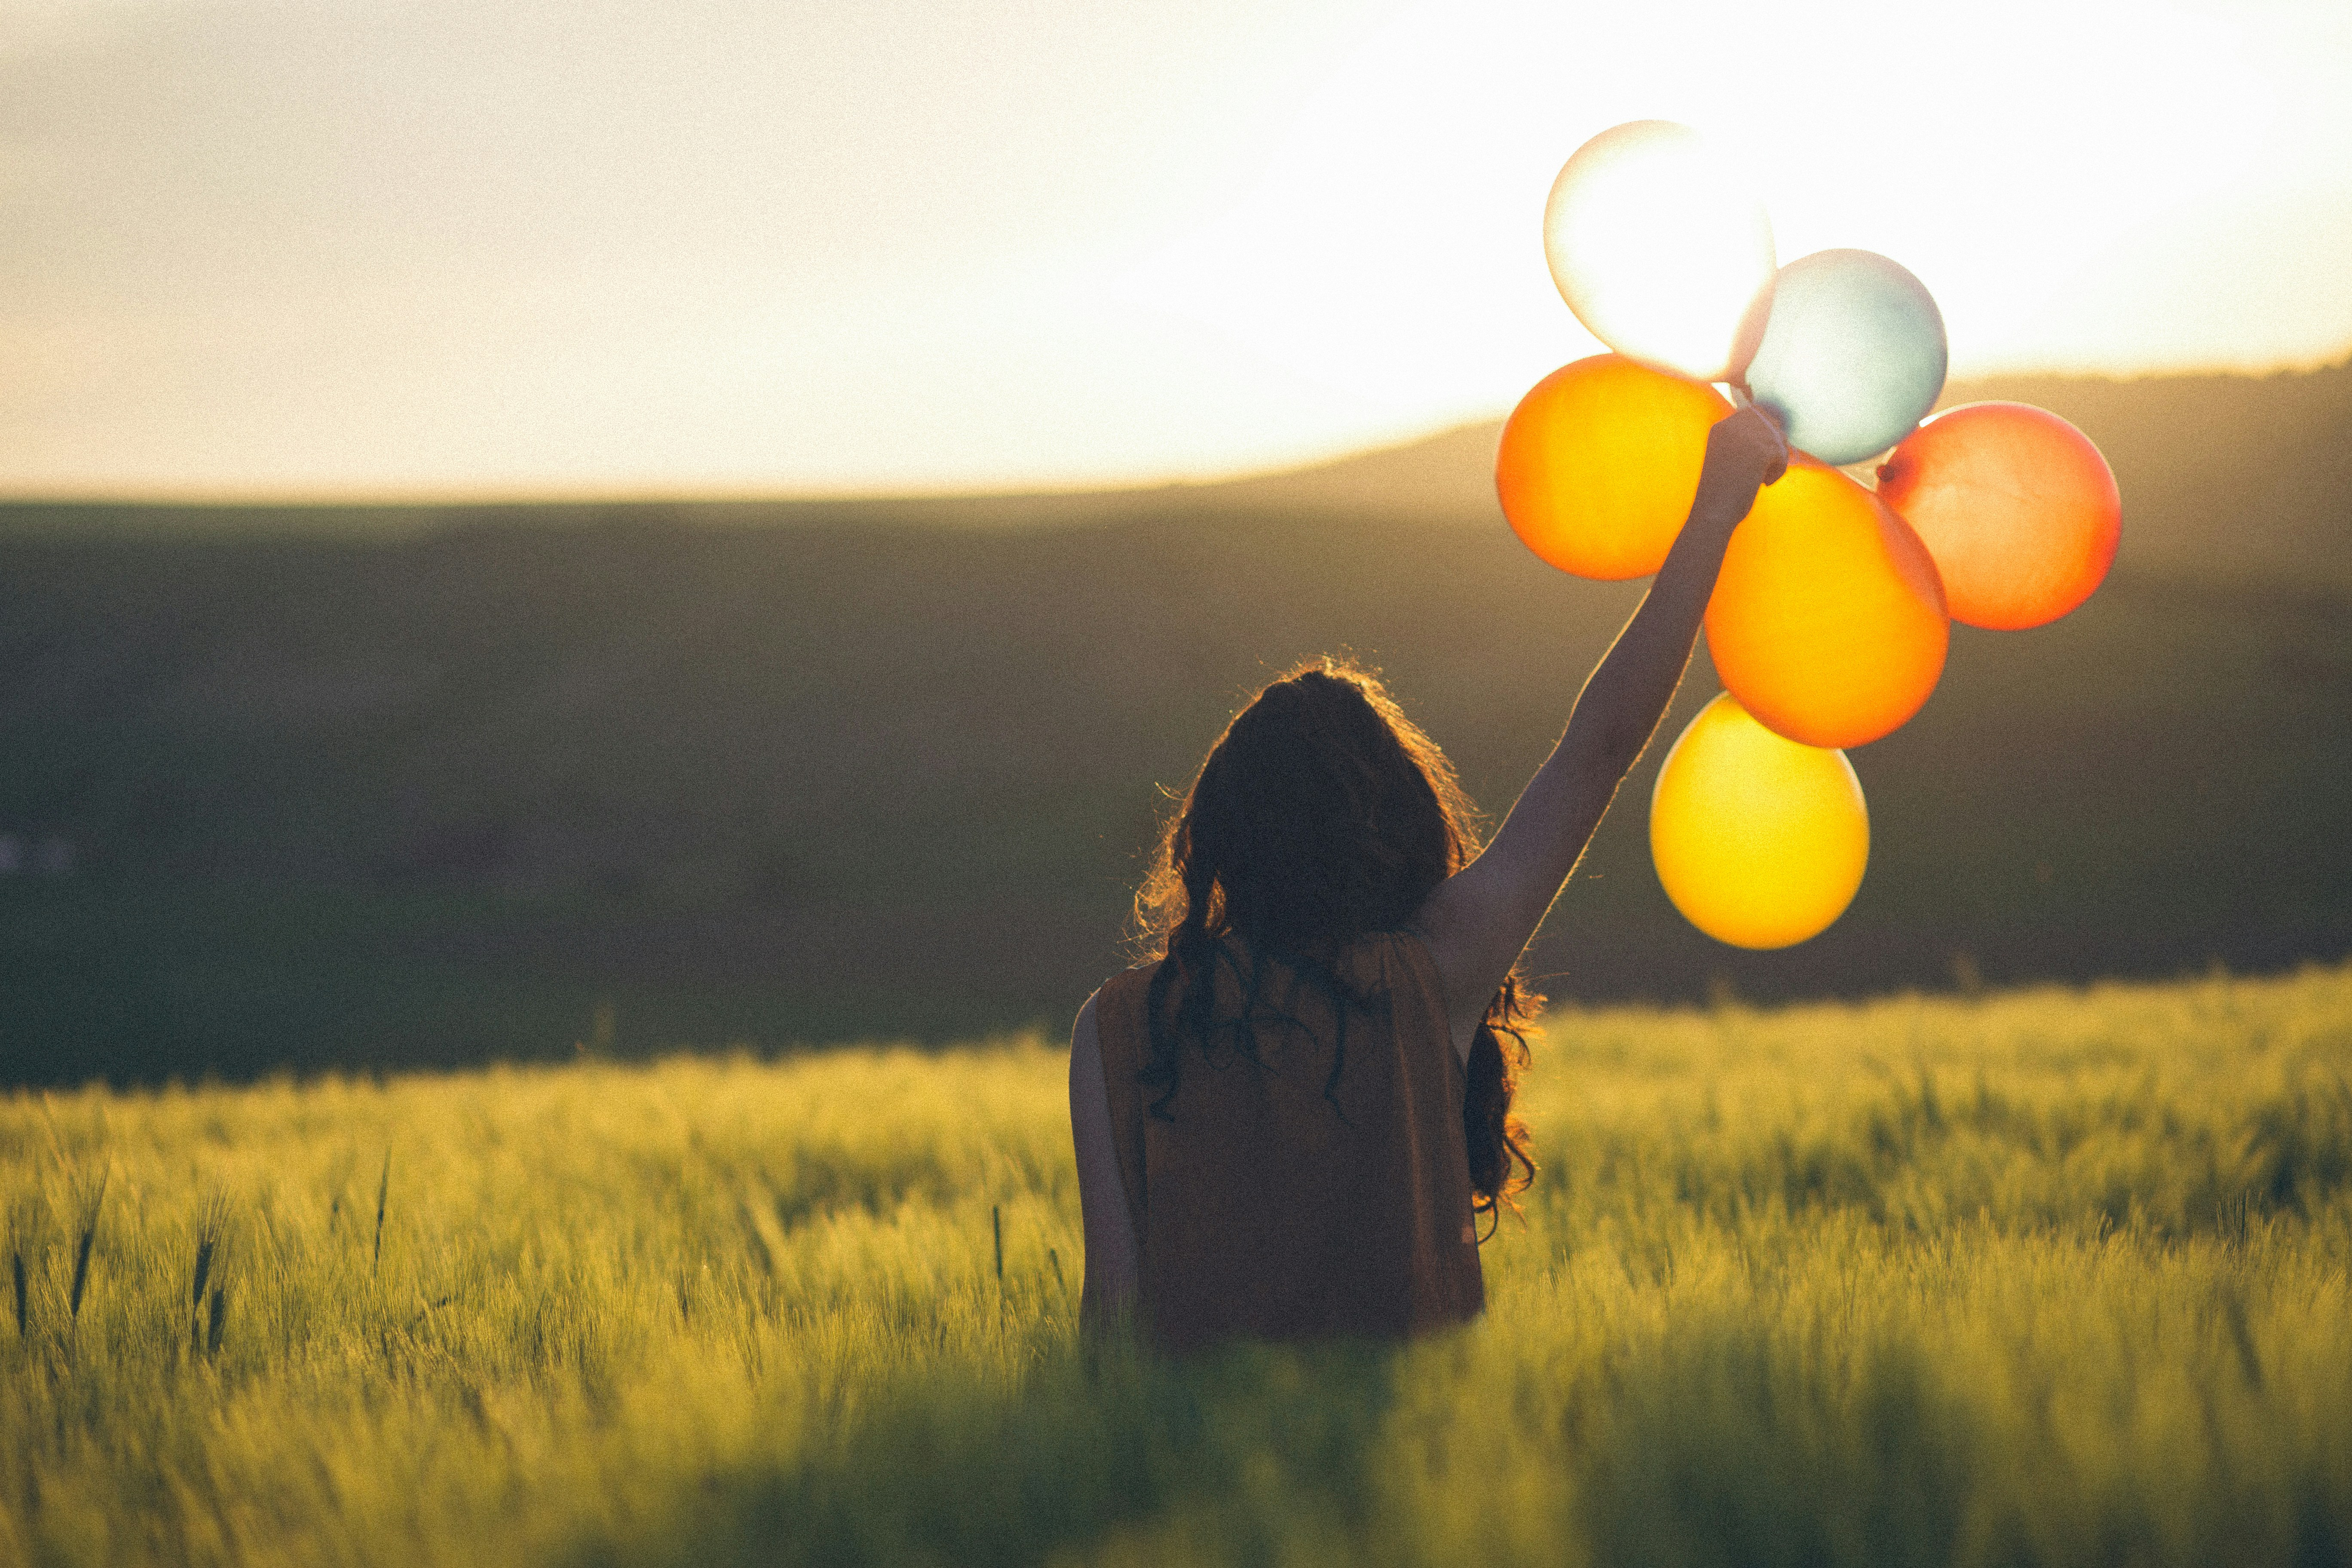
\includegraphics[width=0.8\textwidth]{happiness_unsplash} 
\end{center}

\begin{itemize}
\item Specify image file path: `happiness_unsplash`
\item Control size with options:  `[width=0.8\textwidth]`
\end{itemize}
\end{frame}


\begin{frame}
\frametitle{Captions and Placement}

\begin{figure}[h!] % 'h!' suggests placement 'here' 
 \centering
 \includegraphics[width=0.8\textwidth]{fig1}
 \caption{A descriptive caption about the image.} 
 \label{fig:diagram} 
\end{figure}
\end{frame}


\begin{frame}
\frametitle{Arranging Multiple Images}

\begin{figure}
 \centering
 \includegraphics[width=0.45\textwidth]{alex-kondratiev-H9t723yPjYI-unsplash} 
 \includegraphics[width=0.45\textwidth]{hans-reniers-lQGJCMY5qcM-unsplash}
 \caption{Images side by side.} 
\end{figure}

\begin{itemize}
\item Consider the `subfigure` package for finer control.
\end{itemize}
\end{frame}


\begin{frame}
\frametitle{In-Text Citations}

Studies show that LaTeX is awesome \cite{lamport1994}.

\begin{itemize}
  \item \cite{key} inserts the citation number.
  \item The 'key' must match an entry in your bibliography.
\end{itemize}
\end{frame}


\begin{frame}
\frametitle{Bibliography Styles}

\bibliographystyle{plain} % Example style 
 % Other styles: unsrt, alpha, abbrv, etc.

\begin{itemize}
  \item Controls the formatting of your reference list.
  \item Experiment to find the style that suits your needs.
\end{itemize}
\end{frame}


\begin{frame}[fragile]
\frametitle{Creating a Bibliography}


\begin{enumerate}
  \item Manually: Use the `thebibliography` environment.
  \item BibTeX:  (Preferred) 
       \begin{itemize}
            \item Maintain a `.bib` file with reference entries.
            \begin{verbatim}
            Use \bibliography{my_bibliography.bib} 
            in your LaTeX document.
            \end{verbatim}
       \end{itemize}
\end{enumerate}


\end{frame}



\begin{frame}
\frametitle{Citation Management Tools}

\begin{itemize}
\item Zotero, Mendeley, EndNote, etc.
\item Help with:
    \begin{itemize}
      \item Collecting references
      \item Generating .bib files
      \item Automatically inserting citations
    \end{itemize}
\end{itemize}
\end{frame}


\begin{frame}
\frametitle{Customizing Styles}
\begin{itemize}
  \item Beamer Themes: Control overall slide appearance.
  \item Use \texttt{\textbackslash textcolor\{color\}\{text\}} for text color changes.
  \item Tweak fonts, spacing, and layout elements for a unique look.
\end{itemize}

\textcolor{blue}{Example: Changing slide title color} 
\end{frame}



\begin{frame}
\frametitle{Macros:}

\newcommand{\myequation}[1]{
  \frac{x^2 + 1}{2}
}

Simplify repetitive tasks:  This equation is \myequation{5}. 
\end{frame}


\begin{frame}
\frametitle{Templates}

\begin{itemize}
\item Pre-designed templates for various document types are available.
\item Find templates for theses, resumes, presentations, etc.
\item Great for saving time and ensuring a polished layout. 
\end{itemize}

\emph{Resources:} Websites like Overleaf have template galleries.
\end{frame}


\begin{frame}
\frametitle{Presentations Beyond Beamer}

\begin{itemize}
\item Other LaTeX classes for slides:
    \begin{itemize}
      \item Prosper
      \item Powerdot
      \item ...
    \end{itemize}
\item Each offers different styles and features. 
\end{itemize}
\end{frame}


\begin{frame}
\frametitle{External Files}

\begin{itemize}
\item \input{main.tex} % Includes content directly
\item \include{beamer_presentation.tex} % Starts on a new page 
\end{itemize}

\emph{Use Cases:} Large documents, collaborations, code examples
\end{frame}


\begin{frame}
\frametitle{Collaboration & Version Control}

\begin{itemize}
\item LaTeX text files are ideal for version control systems (like Git).
\item Online tools (e.g., Overleaf) enable real-time collaborative editing - My Recommendation
\end{itemize}
\end{frame}


\begin{frame}
\frametitle{Recap}

\begin{itemize}
\item LaTeX is a powerful typesetting system.
\item Focuses on structure and high-quality output.
\item Handles equations, tables, citations, and more.
\item Customizable and perfect for complex documents. 
\end{itemize}
\end{frame}

\begin{frame}
\frametitle{Where to Learn More}

\begin{itemize}
\item The Not So Short Introduction to LaTeX 2e 
        (https://tobi.oetiker.ch/lshort/) 
\item Overleaf's Learn LaTeX in 30 minutes tutorial (https://www.overleaf.com/learn)
\item CTAN (The Comprehensive TeX Archive Network)  (https://ctan.org/)
\item TeX Stack Exchange (https://tex.stackexchange.com/)
\end{itemize}
\end{frame}


\begin{frame}
\frametitle{Thank You! Questions?}

\begin{center}
\includegraphics[width=0.65\textwidth]{jon-tyson-hhq1Lxtuwd8-unsplash} % Placeholder - add an image related to questions
\end{center}
\end{frame}

\end{document}
